


\subsection{Inverted F-antenna}\label{sec:ifa_sim}




The inverted F-antenna (IFA) is modeled in Ansys HFSS as shown in \autoref{fig:ifa}. Its material is copper. It is positioned at the center of the TEM cell, mounted at the top surface. The 5\,mm long wire points towards waveport 2. The excitation is a modal wave port. With a maximum dimension of 5\,mm, the antenna is electrically small for a frequency of up to 6\,GHz, at which it will be a tenth of the wavelength. In this simulation, the antenna is investigated for the frequency of 100\,MHz to 1\,GHz. The TEM cell has a width of 40\,mm and a height of 24\,mm and an impedance of $\sim50\,\Omega$. The goal is to find equivalent dipole moments of the antenna. 


\begin{figure}[h]
    \centering
    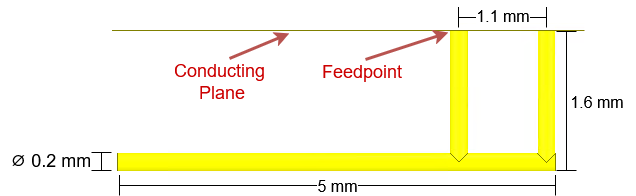
\includegraphics[width=0.75\linewidth]{Documentation//content//30_simulations//img/inverted_f_antenna.png}
    \caption{Inverted F-antenna used in the simulation}
    \label{fig:ifa}
\end{figure}

The coupling between the antenna and the two ports of the TEM cell are described by S-parameters, specifically the forward transmission coefficients $S_{\mathrm{A1}}$ and $S_{\mathrm{A2}}$. \autoref{fig:antenna_waveport1_sparams} shows the magnitude of this coefficient, which is the same for the antenna to both ports ($|S_{\mathrm{A1}}|=|S_{\mathrm{A2}}|$). 
 

\begin{figure}[h]
    \centering
    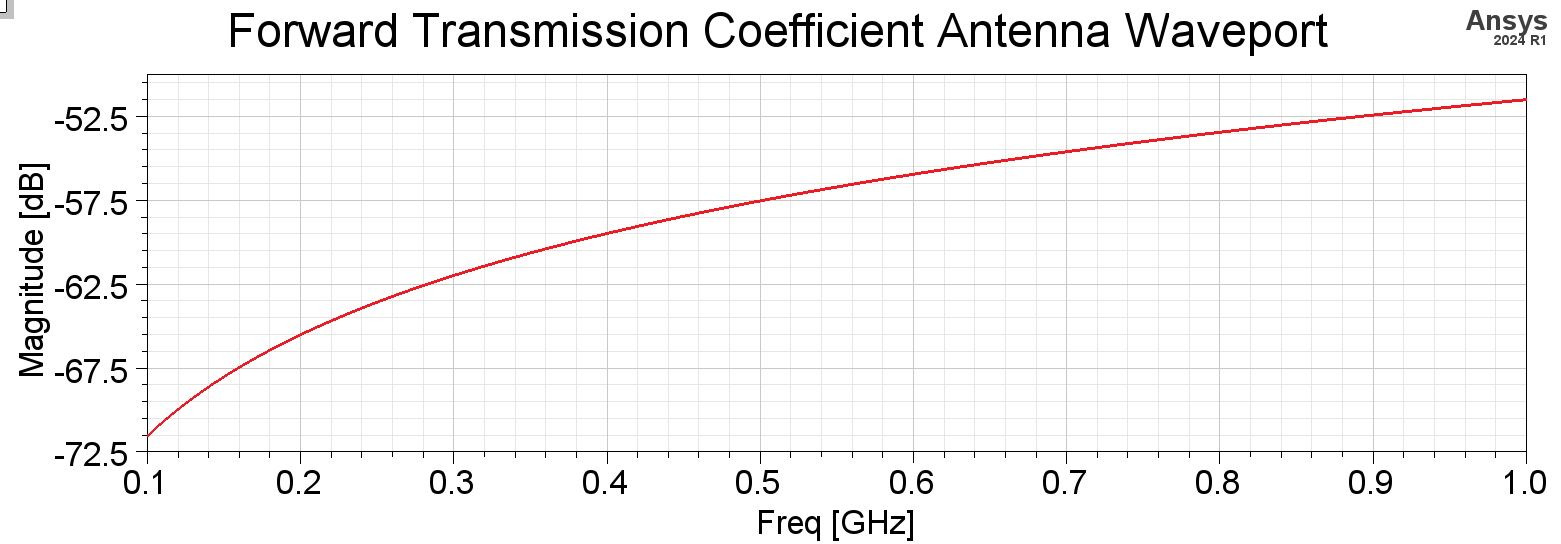
\includegraphics[width=1\linewidth]{Documentation//content//30_simulations//img/antenna_waveport1_sparams.png}
    \caption{S-parameter describing coupling of antenna to waveport 1}
    \label{fig:antenna_waveport1_sparams}
\end{figure}

\begin{equation}
    P_{\mathrm{Antenna}}=\frac{P_{\mathrm{Out1}}}{10^{|S_{\mathrm{A1}}|/10}}=\frac{P_{\mathrm{Out2}}}{10^{|S_{\mathrm{A2}}|/10}}
    \label{eqn:power_antenna}
\end{equation}


\autoref{eqn:power_antenna} describes the relation between the input power at the antenna and the measured output power of the TEM cell. It is defined by the magnitude of the forward transmission coefficients.

\begin{equation}
    \iint_A \mathbf{e_0} \times \mathbf{h_0} \cdot\mathrm{d}\mathbf{A} = 1
    \label{eqn:normalization of fields}
\end{equation}

\autoref{eqn:normalization of fields} shows that the electric field $\mathbf{e_0}$ and magnetic field $\mathbf{h_0}$ are normalized to $1\,\sqrt{\mathrm{W}}$. The surface area $A$, over which the fields are integrated, is that of the output ports of the TEM cell. The field can be linearly scaled by the complex coefficients $a$ and $b$, which has been described in \autoref{eqn:modal_superposition1} and \autoref{eqn:modal_superposition2}. Only one pair of such coefficients is needed, since only the TEM mode is considered.

The coefficients $a$ and $b$ have the unit $\sqrt{\mathrm{W}}$. The fields $\mathbf{e_0}$ and $\mathbf{h_0}$ are not known over the whole area. However, the electric field $\mathbf{e_0}$ has only to be known at one specific point in order to determine the equivalent dipole moments, as will be shown here. The normalization condition therefore leads to an output power equal to $|a|^2/2$ or $|b|^2/2$, respectively, which was also found in \cite{4091811}.

\begin{subequations}
\begin{equation}
    P_{\mathrm{out1}}=\iint_A \langle \mathbf{S} \rangle \cdot \mathrm{d}\mathbf{A}= \iint_A \frac{1}{2} \, \Re \{ \left(a\cdot \mathbf{e_0}\right) \times \left(a\cdot \mathbf{h_0}^*\right) \}\cdot \mathrm{d}\mathbf{A} = \frac{|a|^2}{2}
    \label{eqn:power_of_poynting1}
\end{equation}
\begin{equation}
    P_{\mathrm{out2}}=\iint_A \langle \mathbf{S} \rangle \cdot \mathrm{d}\mathbf{A}= \iint_A \frac{1}{2} \, \Re \{ \left(b\cdot \mathbf{e_0}\right) \times \left(b\cdot \mathbf{h_0}\right)^* \}\cdot \mathrm{d}\mathbf{A} = \frac{|b|^2}{2}
    \label{eqn:power_of_poynting2}
\end{equation}
\end{subequations}



The phase shifts of $S_{\mathrm{A1}}$ and $S_{\mathrm{A2}}$ differ, which is shown in \autoref{fig:phase_shift_waveports_ifa}. The difference of these phase shifts influences the quantity of magnetic dipole moment and electric dipole moments. A large phase shift indicated a large magnetic dipole moments compared to the electric dipole moment, and vice versa. The large difference in phase shifts in \autoref{fig:phase_shift_waveports_ifa} lets one expect the first case. However, the phase shift does not influence the overall output power. It is incorporated into the coefficients $a$ and $b$, by multiplying the term $e^{\mathrm{i}\varphi_{a}}$ or $e^{\mathrm{i}\varphi_{b}}$ to their magnitude. The phase shift of each port is then implemented by $\varphi_{a}$ at the port of the coefficient $a$, and by $\varphi_{b}$ at the port of the coefficient $b$. 

The Poynting vector is periodic from $-\pi/2$ to $\pi/2$, hence any phase difference above that value must be corrected by adding $\pi$ to it. 

\begin{figure}[h]
    \centering
    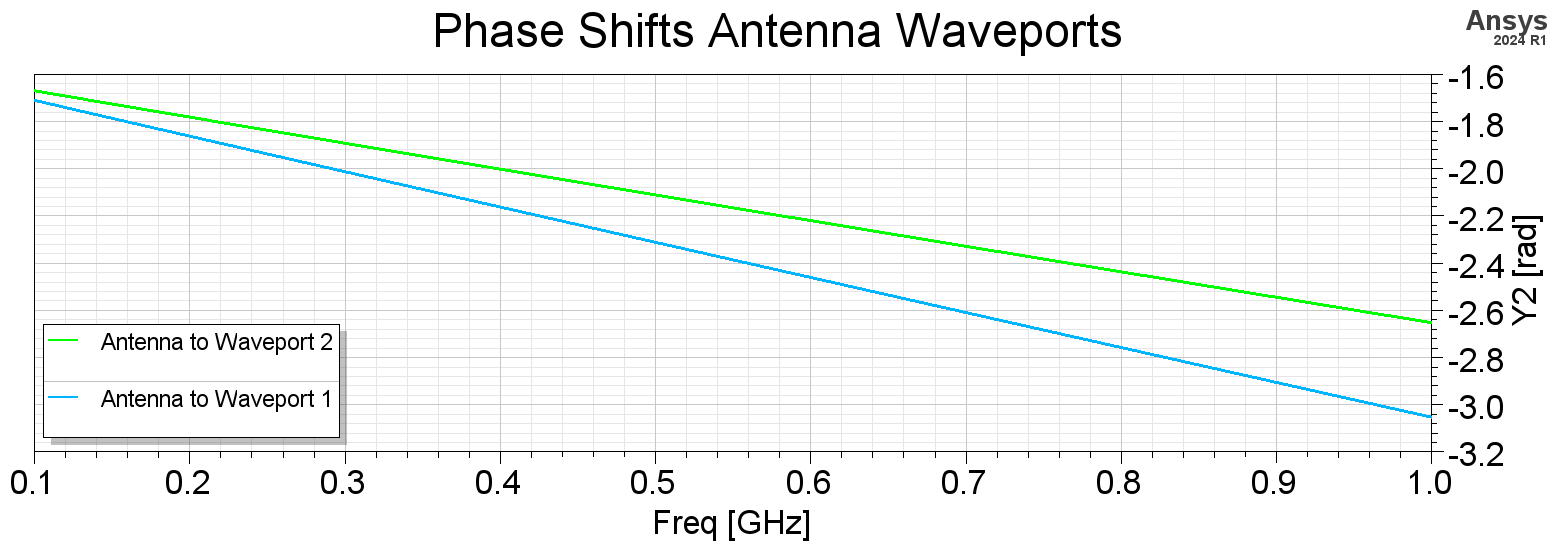
\includegraphics[width=1\linewidth]{Documentation//content//30_simulations//img/Phase Shift Waveports.png}
    \caption{Phase of S-parameters from antenna to waveport 1 and 2}
    \label{fig:phase_shift_waveports_ifa}
\end{figure}

The output power of each port is then derived through \autoref{eqn:power_of_poynting1} and \autoref{eqn:power_of_poynting2}. So if $|a|=|b|=1$, then the electric field $\mathbf{e_0}$ may be measured, when the output power at one port is $\frac{1}{2}\,\mathrm{W}$. Because it is assumed that the TEM cell contains only waves in the TEM mode, the normalization of the electric and magnetic fields can be used to simplify the calculations.

\begin{equation}
    \mathbf{e_0}\times\mathbf{h_0}=\Re\{\mathbf{e_0}\times\mathbf{h_0}^*\} \quad\text{for TEM mode}
    \label{eqn:equivalent_tem}
\end{equation}

\todo{Problem with large TEM cell: Formula does not work for large frequencies. The field distributes around the port. Describe this. Error grows with frequency}

By using \autoref{eqn:mag_dipole_moment_tem} and \autoref{eqn:dipole_tem_waves}, the equivalent dipole moments are derived. Because of Lorentz reciprocity theorem, only fields aligned with the dipole moments get to the output ports. Since only the TEM mode propagates, only the electric dipole moment in z-direction and the magnetic dipole moment in y-direction influence the fields. If higher order modes can propagate, the other dipole moments become relevant, too.
\todo{Einheitliches Koordinatensystem definieren}



\begin{equation}
    m_{\mathrm{e}}=\frac{a+b}{e_{0,z}}
    \label{eqn:ifa_me}
\end{equation}

\begin{equation}
    m_{\mathrm{m}}=\mathrm{i}\frac{a-b}{k_0  e_{0,z}}
    \label{eqn:ifa_mm}
\end{equation}

By adding or subtracting the coefficients $a$ and $b$, the dipole moments are expressed into the handy \autoref{eqn:ifa_me} and \autoref{eqn:ifa_mm}. There, $k_0=\frac{2\pi}{\lambda}$ is the free space wave number and $e_{0,z}$ is the normed electric field in z-direction at middle height between septum and the upper wall of the TEM cell. However, the height of the measurement point is not important, as the electric field is uniformly distributed along the z-axis. Additionally, the x- and y-components of the electric field $\mathbf{e_{0}}$ are zero, which leads to these equations. The dipole moments $m_{\mathrm{e}}$ and $m_{\mathrm{m}}$ are defined to be in the center of the TEM cell, at middle height. If they are shifted in any direction, their approximation would not hold true anymore.

\begin{figure}[h]
    \centering
    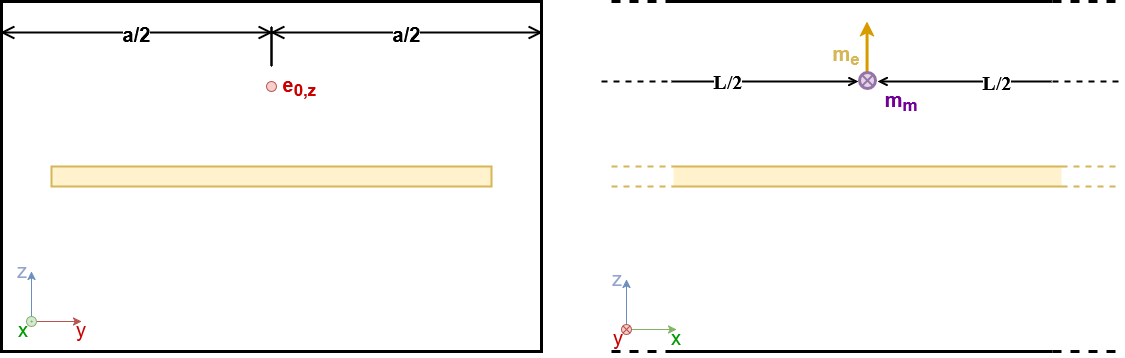
\includegraphics[width=1\linewidth]{Documentation//content//30_simulations//img/sketch_dipoles_tem_cell.png}
    \caption{Dipole moments and measurement point of $e_{0,z}$ in TEM cell}
    \label{fig:sketch_dipoles_tem_cell}
\end{figure}

\autoref{fig:sketch_dipoles_tem_cell} shows the measurement point of $e_\mathrm{0,z}$. This wouldn't work if the magnetic and electric dipole wasn't defined to be exactly at a height of $b/4$, at dead center. The Lorentz Reciprocity theorem used to derive the formulas take the cross product of the electric field traveling to one output port with the magnetic field caused by the dipole, minus the magnetic field traveling to the same output port minus the electric field caused by the dipole. Since the dipoles are in dead center, the electric field caused by the dipole does only have a z-component, and the magnetic field caused by the dipole only a y-component. If this was not the case, the other components would have to be taken into account of the fields at the test point. They would already have disappeared at the output ports due to the long travel, and the Lorentz Reciprocity theorem becomes more cumbersome to use. By placing the dipoles in dead center, it is possible to measure the electric field at the output port and normalize it to $\frac{1}{2}\,\mathrm{W}$.

\todo{Write clearer. And put into theoretical part.}

Using \autoref{eqn:magn_current_curr_loop} the magnetic dipole moment can be expressed as a magnetic current. The resulting $m_{m,mag}$ is shown in \autoref{eqn:m_mymag_ifa}. The phase shift between the magnetic and electric dipole moments $m_{\mathrm{ez}}$ and $m_{\mathrm{my,mag}}$ is always $\frac{\pi}{2}$, which generates the desired TEM wave pattern.

\begin{equation}
    m_{\mathrm{m,mag}}=\mathrm{i}m_{\mathrm{m}}\omega\mu_0
    \label{eqn:m_mymag_ifa}
\end{equation}

The antenna may then be replaced with those two dipole excitations in the center of the upper half of the TEM cell. The magnitude and phase of the fields, as well as the output powers, should remain the same as in the case with the antenna. The phase shift may be determined by measuring the phase shifts of the electric fields at both output ports. When applying this described method in a measurement with a real TEM cell, the phase shift may be found by adding and subtracting the output powers of both ports, as is shown in \cite{Sreenivasiah_Chang_Ma_1981}.

\begin{figure}[h]
    \centering
    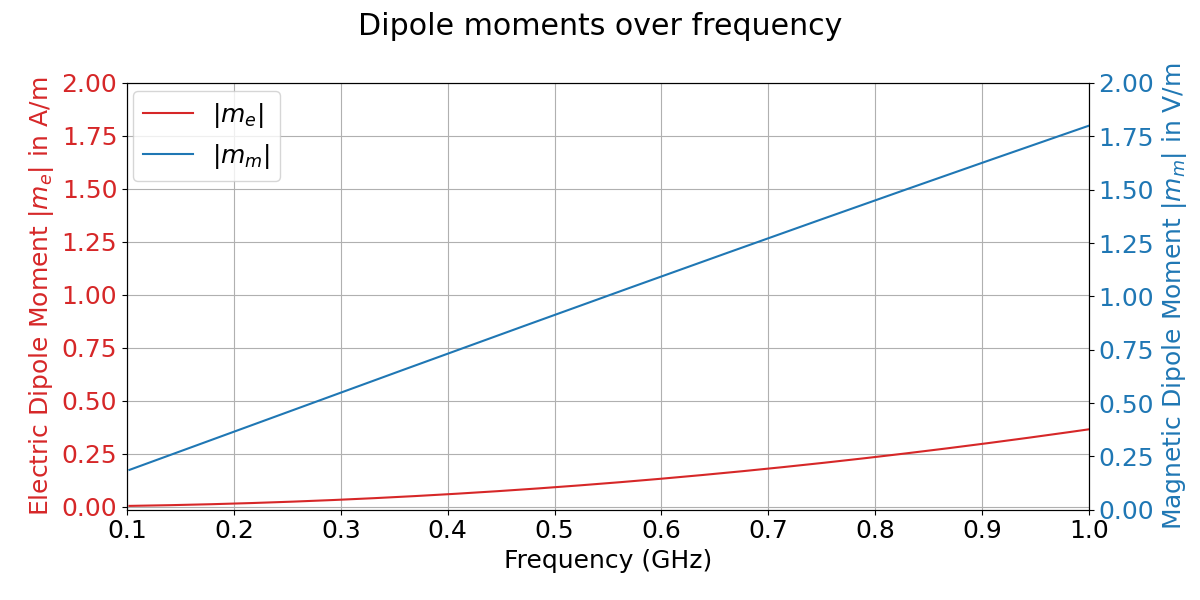
\includegraphics[width=1\linewidth]{Documentation/content/30_simulations/img/dipole_moments_over_freq_ifa.png}
    \caption{Dipole moments over frequency}
    \label{fig:dipole_moments_over_freq_ifa}
\end{figure}

\autoref{fig:dipole_moments_over_freq_ifa} shows the dipole moments over frequency. The electric dipole moment $m_e$ has been normalized to the free-space wave impedance of $377\,\Omega$ to make the dipole moments comparable. The antenna input power has been set to 142588.47\,W, because this leads to an output power of 1\,W at a frequency of 1\,GHz. The magnetic dipole moment is much larger than the electric dipole moment, because the current loop of the antenna is aligned with the TEM cell's magnetic fields, but the line current is not with the TEM electric fields. The magnetic dipole moments rises linearly with the frequency, which is equal to a quadratic increase of power. Only the TEM modes has been considered in the simulation, as other modes disturb the calculations. 

The electric field $\mathbf{e_0}$ is approximated with \autoref{eqn:ifa_e_field_approx} for the purpose of interpolation over frequencies and analytical analysis. The constant $u$ is a scaling factor, which must be adjusted to fit the real electric field values. In this case, this constant equals $u=820.34$. The left-hand side term $|a|\cdot e_{0,z}$ is the overall electric field at the measurement point according to \autoref{eqn:modal_superposition1}. \autoref{fig:output_power_e_fields_over_freq_ifa} shows the resulting plot. 

\begin{equation}
    |a|\cdot e_{0,z}=\sqrt{2P_\mathrm{Out}}\cdot e_{0,z}=u\sqrt{P_\mathrm{Out}}\,\mathrm{\frac{V}{m\cdot\sqrt{W}}}
    \label{eqn:ifa_e_field_approx}
\end{equation}

\begin{figure}[h]
    \centering
    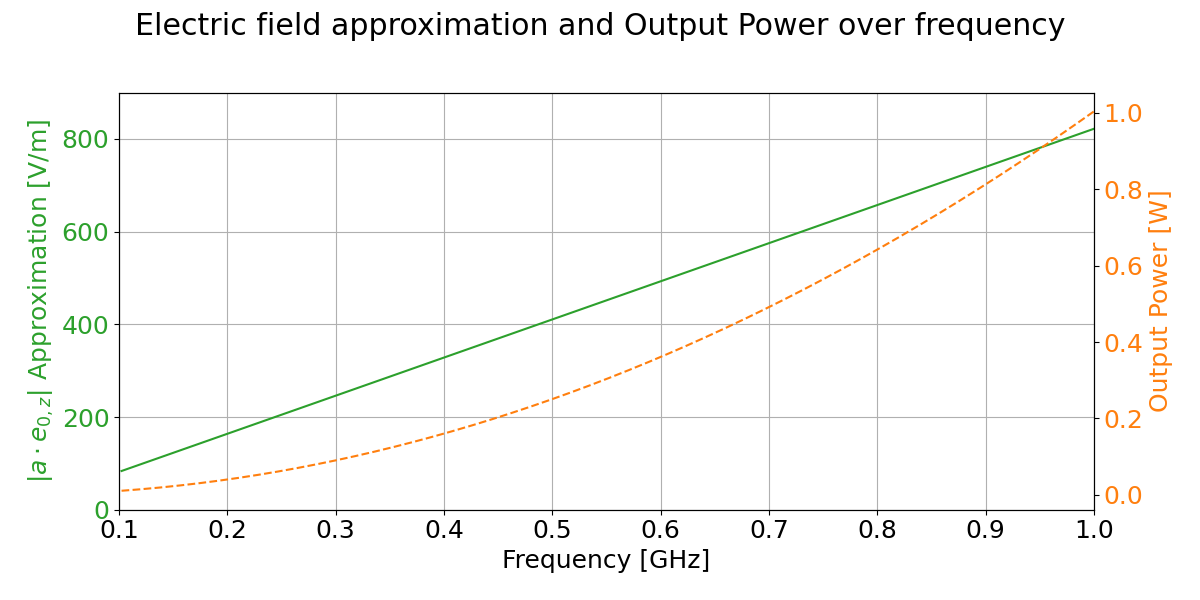
\includegraphics[width=1\linewidth]{Documentation//content//30_simulations//img/output_power_e_fields_over_freq_ifa.png}
    \caption{Output power and electric field over frequency}
    \label{fig:output_power_e_fields_over_freq_ifa}
\end{figure}

The electric field can also be approximated by \autoref{eqn:e_field_at_one_point}, where $b/2=12\,\mathrm{mm}$ is half the height and $Z_\mathrm{W}\approx50\,\Omega$ is the impedance of the TEM cell. This works for TEM cells with thin septum. The constant $u$ can be adjusted to fit this equation. The term $\sqrt{2}$ is needed to convert the effective value of the electric field into its magnitude.

\begin{equation}
    |a|\cdot e_{\mathrm{0,z}}=\frac{\sqrt{2\cdot P_\mathrm{Out}\cdot Z_\mathrm{W}}}{b/2}
    \label{eqn:e_field_at_one_point}
\end{equation}

\todo{Repeat for different orientations? Change variable name: TEM cell height.}

The magnetic coupling with the septum happens due to the alignment of the current loop with the magnetic field of the dominant TEM mode. The antenna is now rotated by 90° around the z-axis, such that the magnetic current loop stands perpendicular to the magnetic TEM fields. \autoref{fig:phase_shift_90_ifa} demonstrates the phase of the S-parameters, describing the coupling of antenna to waveport 1 and 2. Since the magnetic dipole moment is responsible for a phase between the ports, \autoref{fig:phase_shift_90_ifa} strongly hints to an absence of it.

\begin{figure}[h]
    \centering
    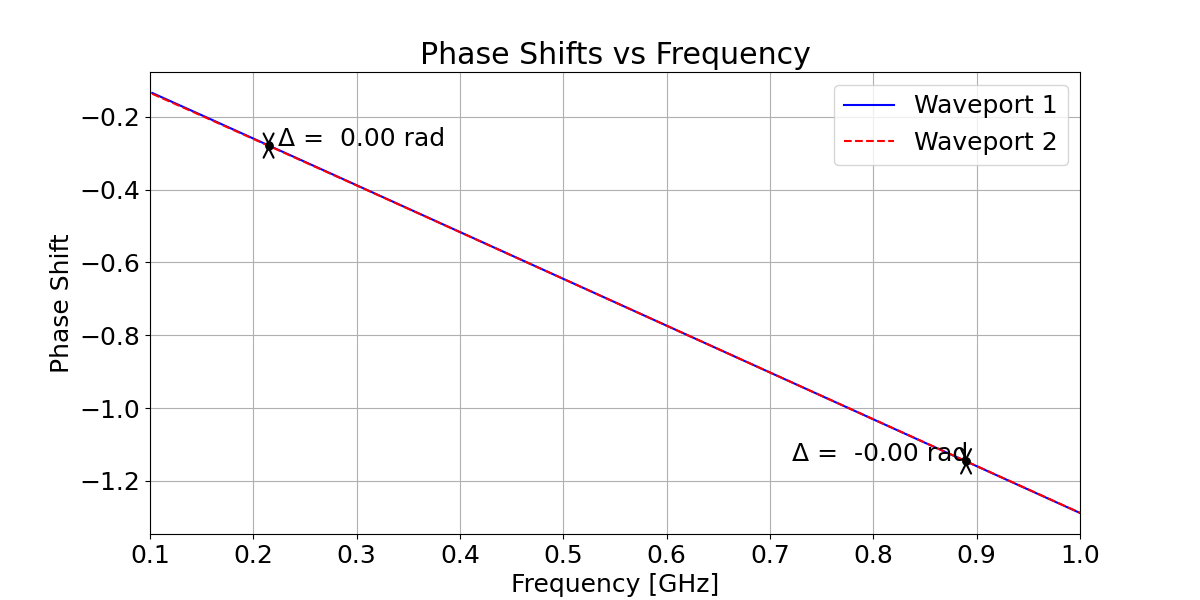
\includegraphics[width=1\linewidth]{Documentation//content//30_simulations//img/phase_shift_90_ifa.png}
    \caption{Phase of S-parameters from rotated antenna to waveport 1 and 2}
    \label{fig:phase_shift_90_ifa}
\end{figure}

\autoref{dipole_moments_ifa_90} shows that the electric dipole moment $m_\mathrm{e}$ has stayed the same, while the magnetic dipole moment became zero. Consequently, the overall power transfer between the antenna and the waveports is also much lower. 

\todo{The same procedure was repeated with different dipole moments positions, for which \autoref{eqn:e0z_mse} worked. Maybe do a general equation for the normalized e-field?}

\begin{figure}[h]
    \centering
    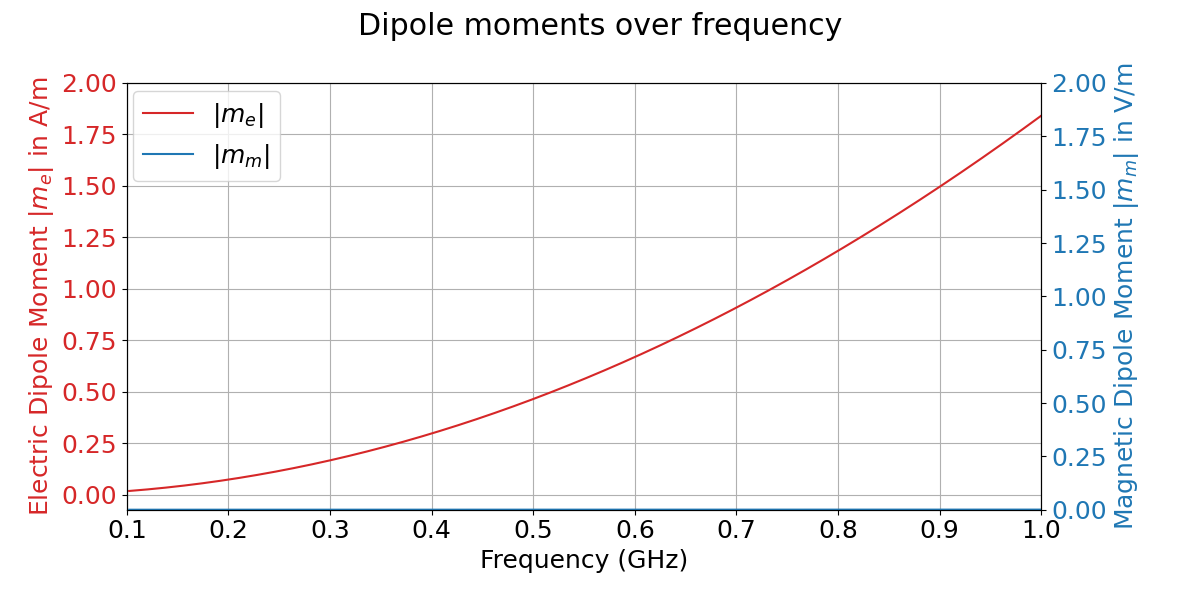
\includegraphics[width=1\linewidth]{Documentation//content//30_simulations//img/dipole_moments_ifa_90.png}
    \caption{Dipole moments of rotated antenna}
    \label{fig:dipole_moments_ifa_90}
\end{figure}


\subsection{Center Fed Monopole Antenna}

The center fed monopole antenna is shown in \autoref{fig:center_fed_monopole}. The conducting plane in \autoref{fig:center_fed_monopole} is on the top side of the TEM cell, thus the image is rotated counter-clockwise by 90 degrees. The electric wire with the length of 5 mm points towards the septum. The 1.1 x 1.6 mm loop is again aligned with the magnetic field lines of the TEM mode. The antenna is fed with a power of $P_\mathrm{Antenna}=127770.39\,\mathrm{W}$, which once more leads to an output power of $P_\mathrm{Out}=1\,\mathrm{W}$ at 1\,GHz at both output ports. 

\begin{figure}[h]
    \centering
    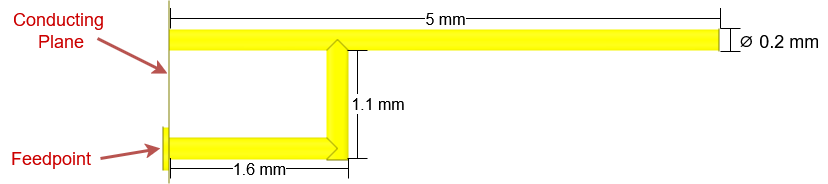
\includegraphics[width=0.75\linewidth]{Documentation//content//30_simulations//img/center_fed_monopole.png}
    \caption{Center fed monopole antenna used in simulation}
    \label{fig:center_fed_monopole}
\end{figure}

The magnitude of $|S_\mathrm{A1}|=|S_\mathrm{A2}|$ in \autoref{fig:forward_coeff_cfm} shows stronger coupling. As will be seen below, this is because of an increased electric dipole moment, while the magnetic dipole moment remained the same. Therefore, the center fed monopole antenna couples well electrically with the TEM cell.

\begin{figure}[h]
    \centering
    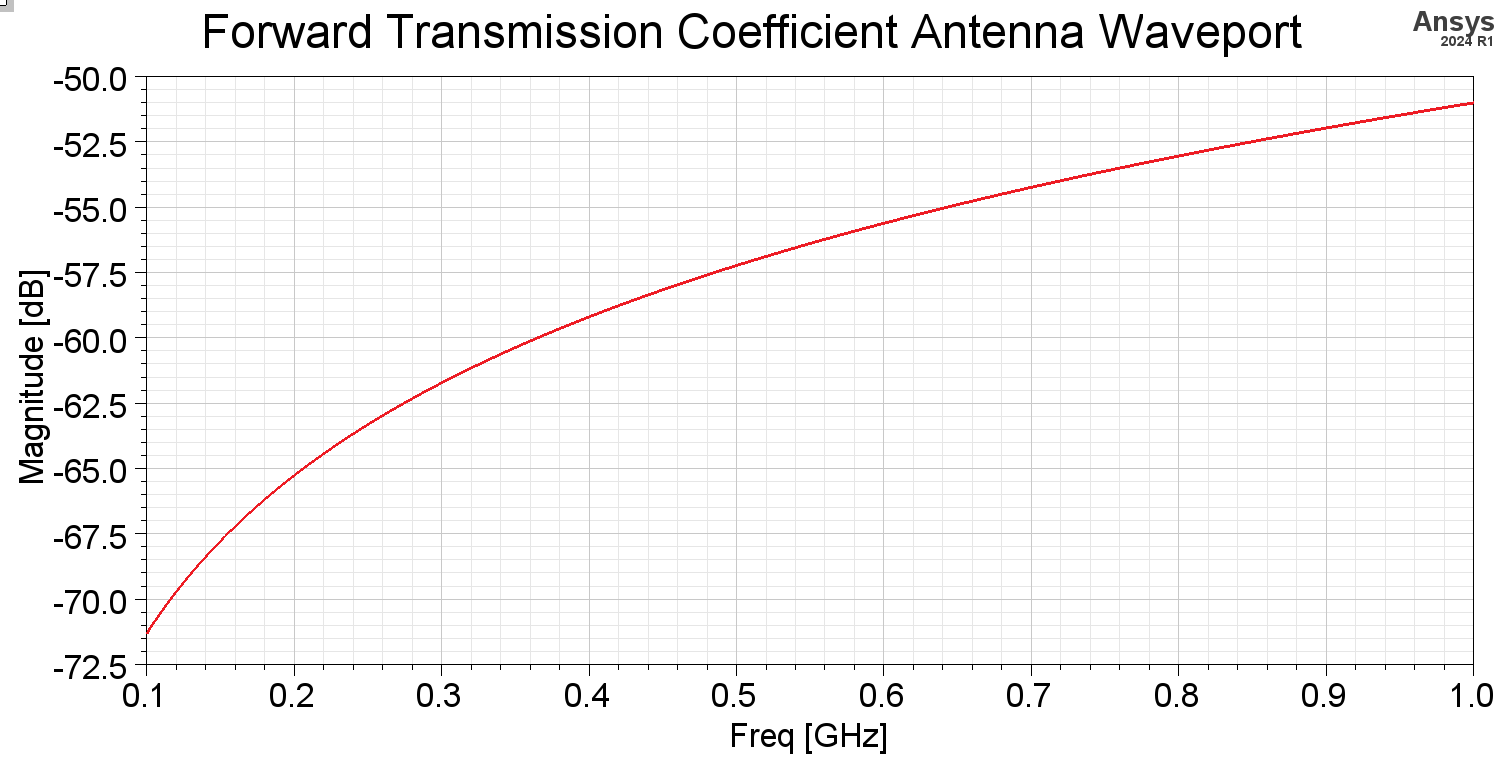
\includegraphics[width=1\linewidth]{Documentation//content//30_simulations//img/forward_coeff_cfm.png}
    \caption{S-parameter describing coupling of antenna to waveport 1}
    \label{fig:forward_coeff_cfm}
\end{figure}

The phase shift in \autoref{fig:phase_shift_cfm} is smaller than in the simulation with the inverted F antenna. This hints to a more influential electric dipole moment than before. This is because of the term $a+b$... When using superposition of each dipole moment...

\begin{subequations}
    \begin{equation}
        c_1 = \sqrt{a^2+b^2+2ab\cos{\left[ (\varphi_a + \varphi_b) / 2 \right]}}
    \end{equation}
        \begin{equation}
        c_2 = \sqrt{a^2+b^2-2ab\sin{\left[ (\varphi_a - \varphi_b) / 2 \right]}}
    \end{equation}
    \begin{equation}
        c_1^2+c_2^2= a^2+b^2
    \end{equation}
\end{subequations}
\todo{not done yet, make it correct}
    

\begin{figure}[h]
    \centering
    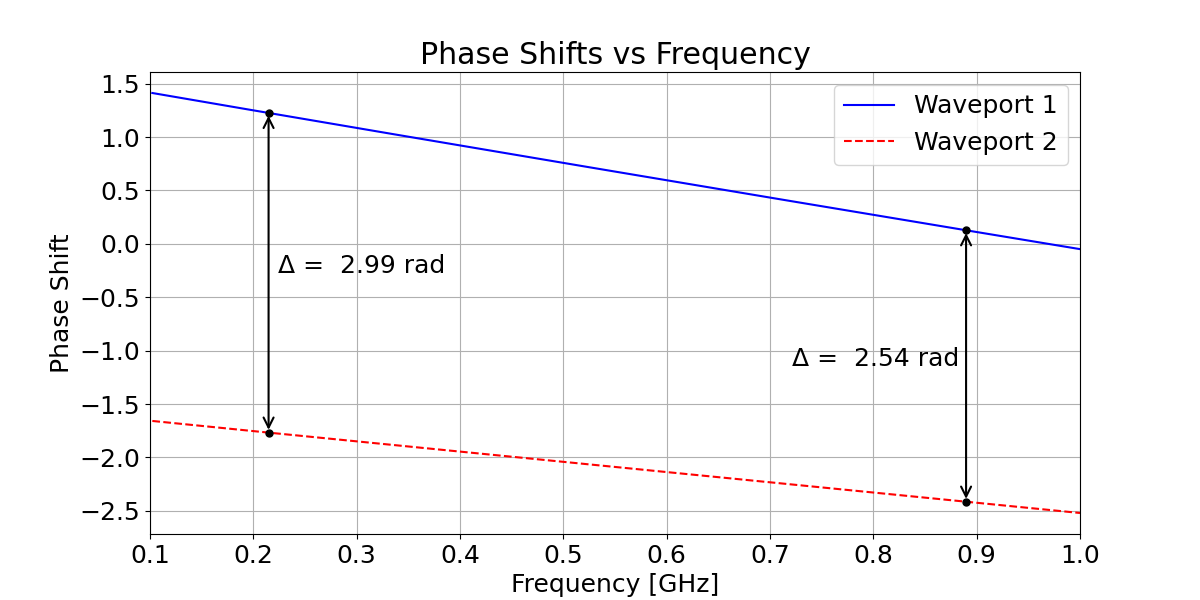
\includegraphics[width=1\linewidth]{Documentation//content//30_simulations//img/phase_shift_cfm.png}
    \caption{Phase of S-parameters from antenna to waveport 1 and 2}
    \label{fig:phase_shift_cfm}
\end{figure}

\autoref{fig:dipole_moment_cfm} shows that the magnetic dipole moments of the inverted F and center fed monopole antennas are equal. This is due to the same size of the current loops. However, the electric dipole moments increased for the center fed monopole antenna. The alignment of the line current with the TEM cell's electric field causes this.

\begin{figure}[h]
    \centering
    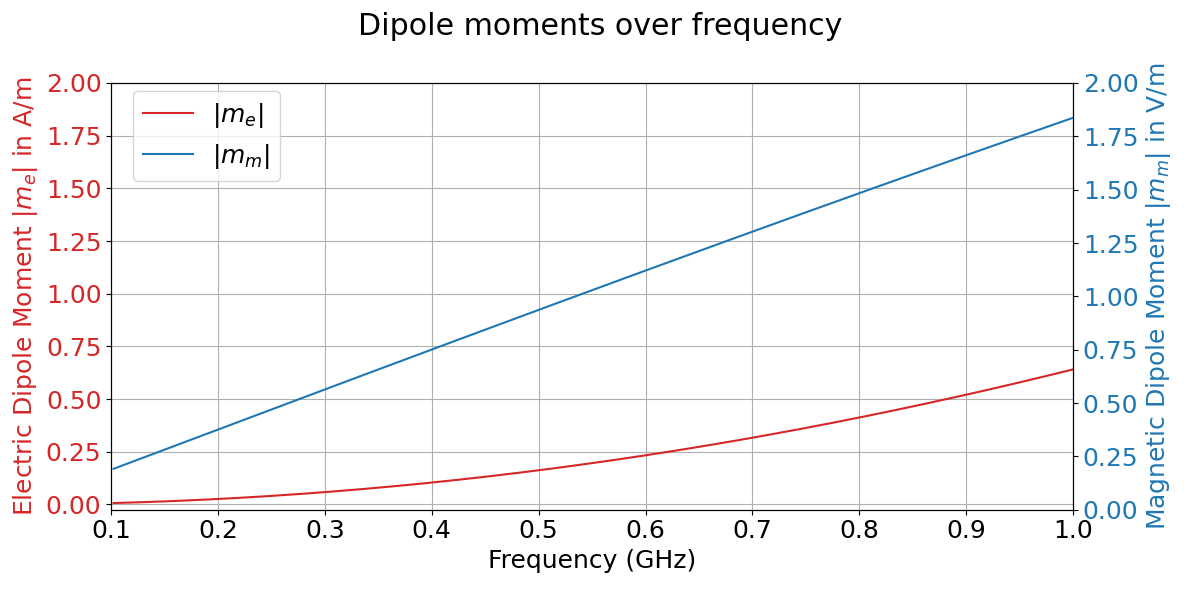
\includegraphics[width=1\linewidth]{Documentation//content//30_simulations//img/dipole_moment_cfm.png}
    \caption{Dipole moments over frequency}
    \label{fig:dipole_moment_cfm}
\end{figure}


The output power has been scaled as in the simulation before. This leads to the same electric field magnitude. Therefore, the electric field and output power over frequency plot are the same as in the case for the inverted F antenna, visible in \autoref{fig:output_power_e_fields_over_freq_ifa}.

\subsection{Offset of source antennas and eddy currents}

Eddy currents occur on the septum. They increase with frequency. When they get too large, the next-order mode starts propagating. Offsetting the antenna / dipole moment in y-direction reduces the amount of influence of the eddy current on the power carrying current in the septum. 

\todo{How does offset influence the eddy currents and the result?}

\subsection{Shielding effectiveness of graphite}

The reference power $P_\mathrm{ref}$ has been set to 1\,W. Using \autoref{eqn:load_power} and the S-parameters from the simulation results, $P_\mathrm{load}$ may be determined. \autoref{fig:se_graphite} demonstrates the shielding effectiveness of graphite in dB $SE_\mathrm{dB}$ over the shielding material thickness. The solution frequency is 500\,MHz. A frequency sweep shows that the reflection coefficient $S_{11}$ does not depend much on the frequency. 

\begin{figure}[h]
    \centering
    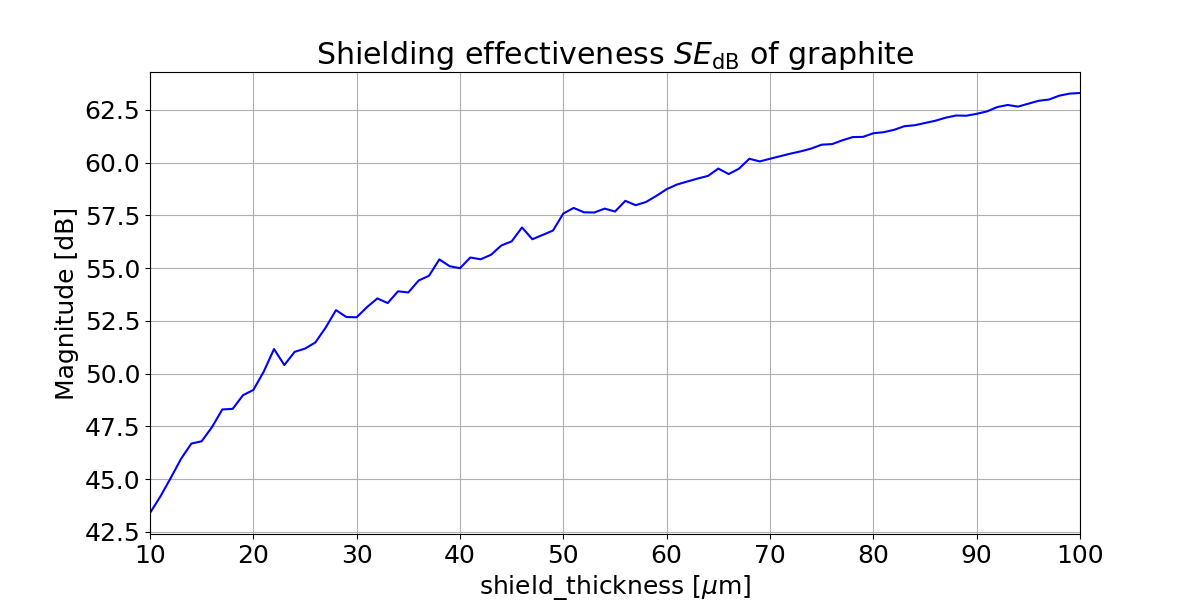
\includegraphics[width=1\linewidth]{Documentation//content//30_simulations//img/se_graphite.png}
    \caption{Shielding effectiveness of graphite}
    \label{fig:se_graphite}
\end{figure}

\todo{I think the low SE in the low shield thicknesses has to do with the false modelling of it in Ansys HFSS.}

The components of $SE_\mathrm{dB}$ are determined according to \autoref{eqn:se_rereflections}. 

\subsection{Shield effectiveness of FR4}

The FR4 has a relative permittivity of $\epsilon_r=4.4$. According to \autoref{eqn:rel_wave_imp}, the relative wave impedance is $Z=0.476$. This leads to a reflection coefficient of $R=-0.355$ by \autoref{eqn:reflection_coefficient_plane_dielectric}.


The reflection coefficient $|S_{11}|=0.045$.
